\documentclass[answers]{exam}
\usepackage[english]{babel}
\usepackage[letterpaper,top=2cm,bottom=2cm,left=3cm,right=3cm,marginparwidth=1.75cm]{geometry}
\usepackage{amsmath, amssymb}
\usepackage{graphicx}
\usepackage{enumitem}
\usepackage{tikz,pgfplots}
\pgfplotsset{compat=1.18}
\usepackage[colorlinks=true, allcolors=blue]{hyperref}

% Header and footer
% \pagestyle{headandfoot}
% \firstpageheader{Universidad de Bolívar}{}{\today}
% \runningheader{Universidad de Bolívar}{}{\thepage}
% \firstpagefooter{}{}{}
% \runningfooter{}{}{}

\begin{document}

\begin{center}
	% \Large\textbf{Cálculo I}\\[1em]
	\large\textbf{Prueba de Calculo}\\[1em]
	% \large Primer Ciclo "A" - Ingeniería de Software\\[1em]
	% \large \today
\end{center}

% \vspace{0.5cm}
% \large\textbf{Estudiante}: Ariel Alejandro Calderón
% \vspace{0.5cm}



	\text{\textbf{Recomendacion general:} Siempre que se pueda, usar el grafico para responder preguntas.}\\
	\text{Algunas preguntas van a requerir esfuerzo extra (analisis matematico)}



\vspace{0.5cm}

\begin{questions}

	
	% Question 1
	\question \large\textbf{Para las siguientes funciones hallar dominio y recorrido:}
	\begin{enumerate}[label=\alph*.]
		\item $\displaystyle f(x) = \frac{\sqrt{x-1}}{x-4} $
		\item $\displaystyle g(x) = \frac{x^3-2x}{x^3} $
	\end{enumerate}
	
	\vspace{0.5cm}
	% Question 2
	\question \large\textbf{Usando las funciones del ejercicio anterior, calcular $(f+g)(x)$ y el dominio de esta funcion:}

	\vspace{0.5cm}
	% Question 3
	\question \large\textbf{Estudiar la biyectividad de $f(x)=\dfrac{\sqrt{x-1}}{x-4}$. Si la funcion es biyectiva, hallar la funcion inversa.}

	\vspace{0.5cm}
	% Question 4
	\question \large\textbf{Estudiar la paridad de $f(x)=\dfrac{x^4+1}{x^2}$.}

	\vspace{0.5cm}
	% Question 4
	\question \large\textbf{Estudiar la monotonia de $f(x)= \dfrac{1}{x^2-3}$.}

	\vspace{0.5cm}

	
\end{questions}

\end{document}
% \begin{solution}
	% 	\begin{minipage}{\textwidth}
	% 		\centering
	% 		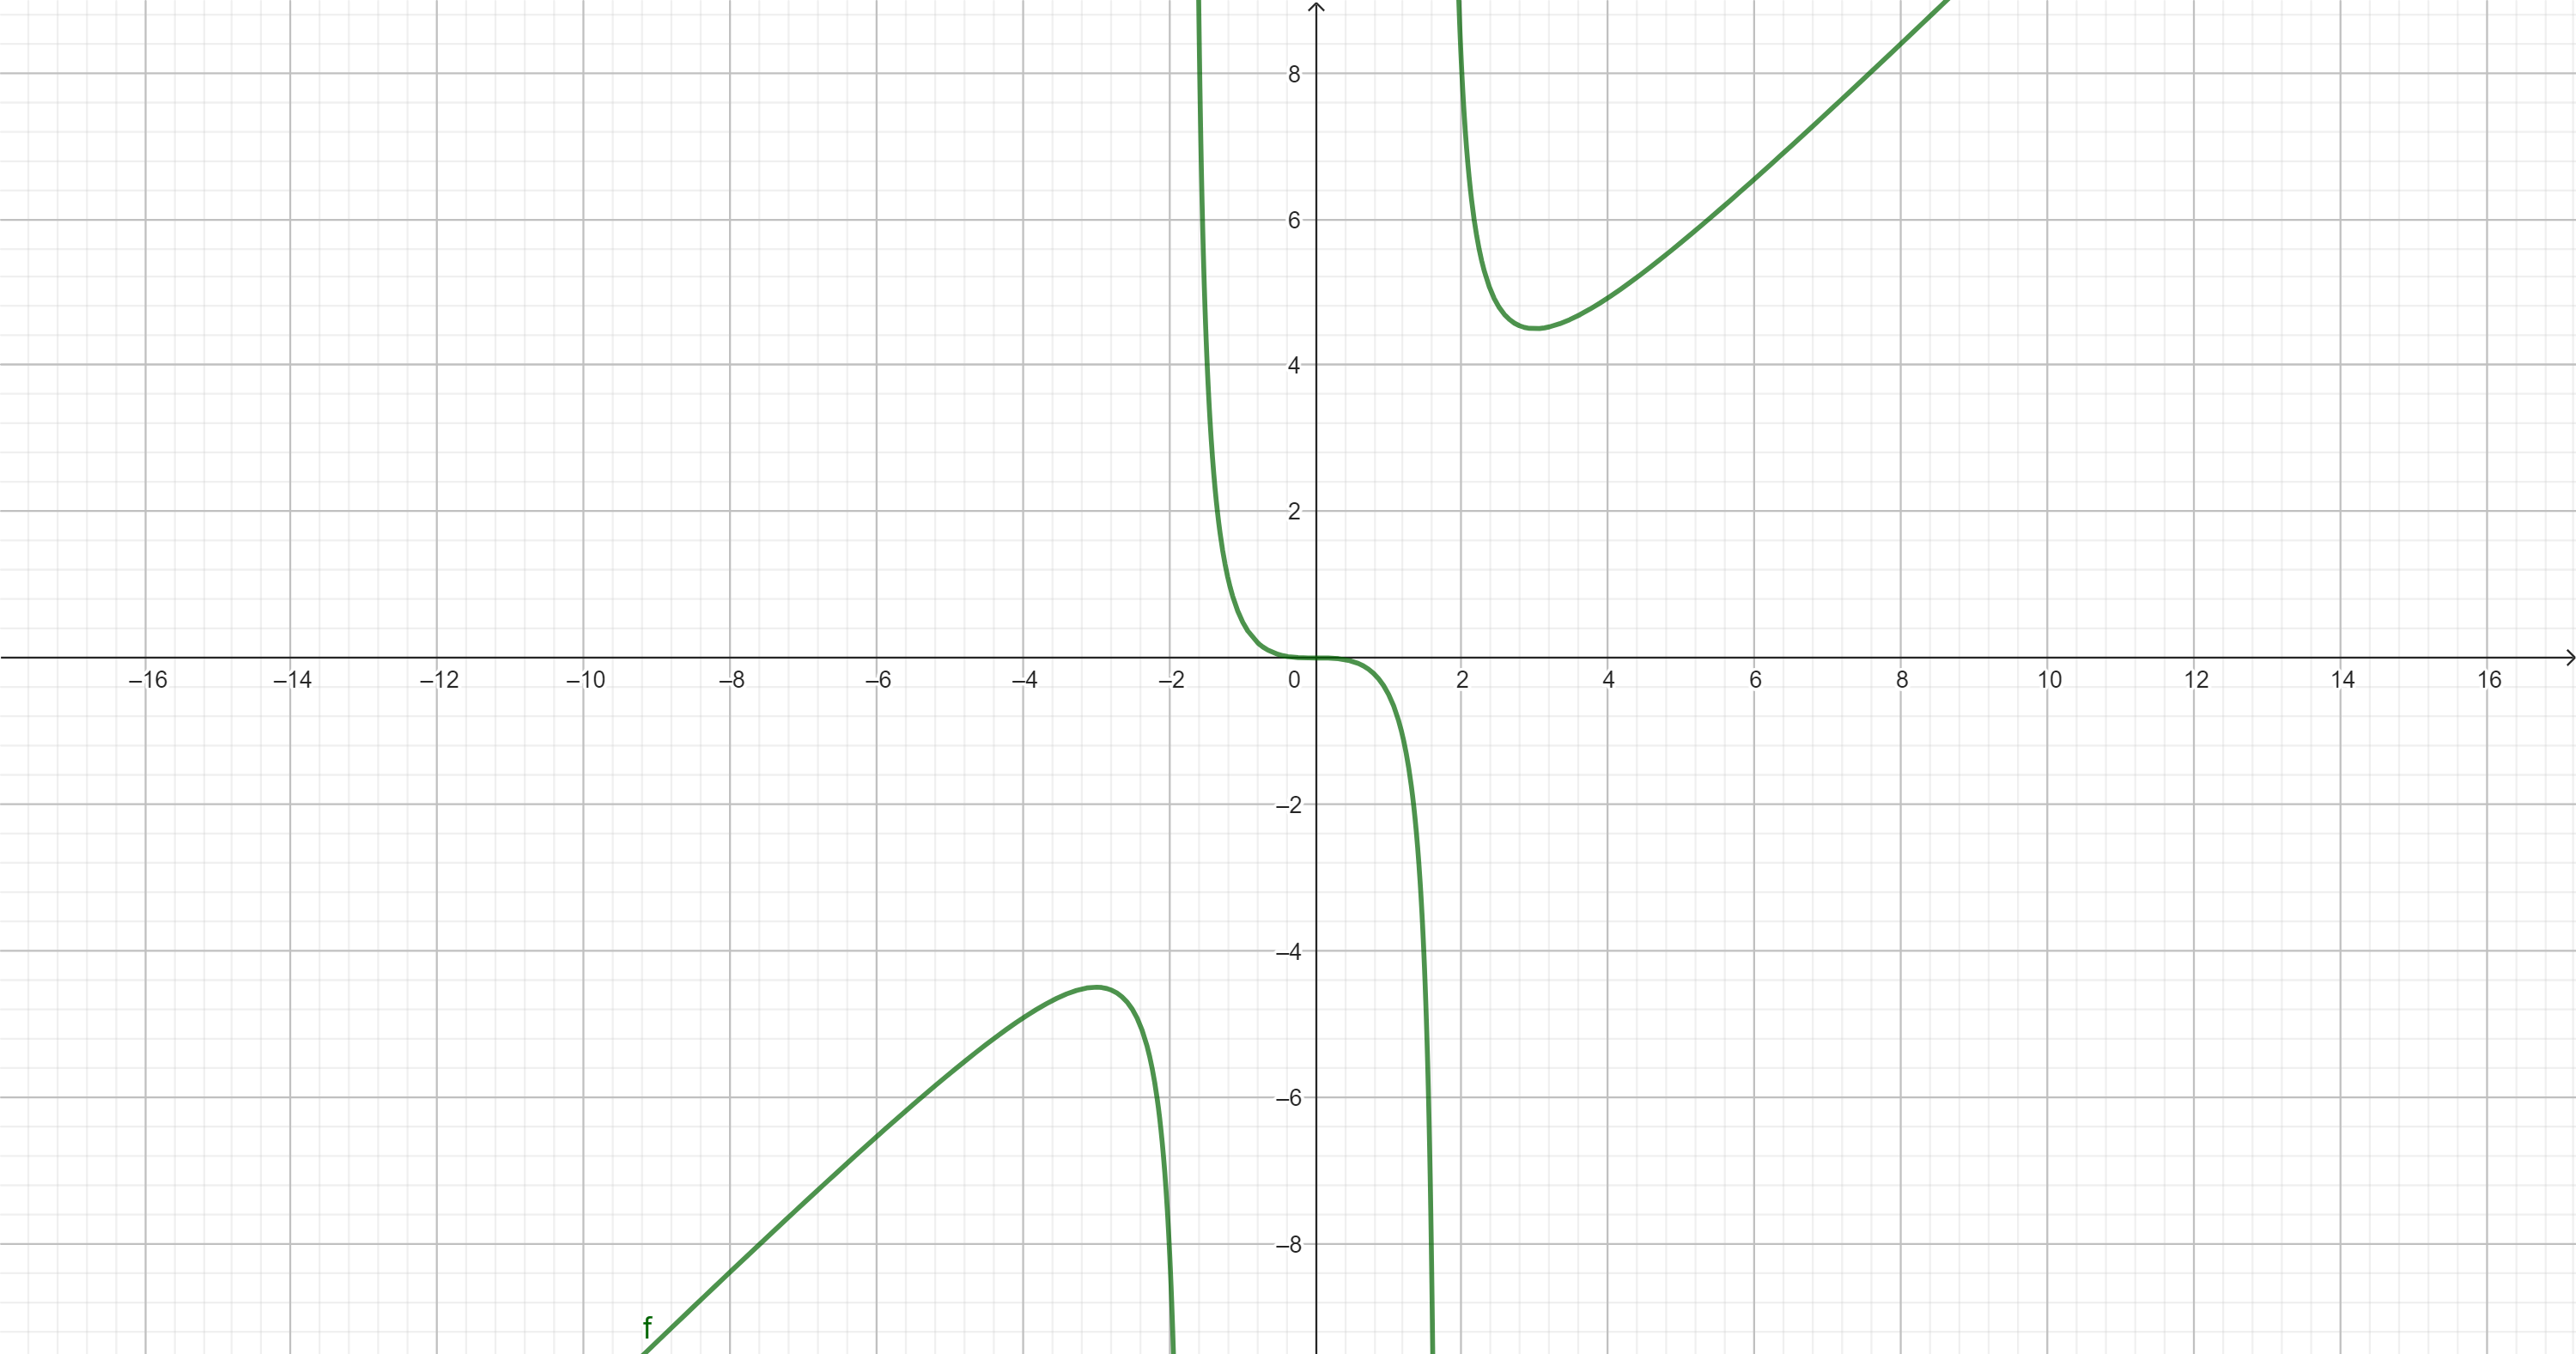
\includegraphics[width=0.9\textwidth]{public/g1.png}\\
	% 	\end{minipage}
	% 	\vspace{0.5cm}
	% \end{solution}